\chapter{Field collection methods}\label{sec:field-collection-methods}
\begin{remark}{Outline}
Previous records were used in conjunction with one off surveys to identify good monitoring locations. When locations were identified a standard programme was initiated. A range of static and dynamic image data were collected during field work but the main body of this research focuses on a method to monitor broad populations of native bees using images of their active nests. This chapter describes the study locations, the methods used to determine the start and end of monitoring seasons, the types of environmental data collected and the tools used to collect data. This chapter also covers the techniques used to manually count active nests and methods used for collecting monitoring images.
\end{remark}

\section{Monitoring locations}\label{sec:monitoring-locations}

\begin{sidewaysfigure}[!htbp]\myfloatalign
\includegraphics[width=0.9\linewidth]{gfx4/map1} \\
\caption[Study locations.]{Google Map~\textcopyright~showing the site locations and photographs of each monitoring area. }\label{fig:locations-map}
\end{sidewaysfigure}

\begin{table}[!htbp]\myfloatalign \caption[Monitoring locations.]{Monitoring locations and  map co-ordinates.}\label{tab:locations} 
\begin{tabular}{lp{1.1in}p{2.1in}}\toprule
Site number & Name & Location \\ \midrule
Site 1 & Mt. Tiger & 35\textdegree 44' 31.9" S, 174\textdegree 25' 18.8" E \\
Site 2 & Mt. Parihaka & 35\textdegree 42' 41.4" S, 174\textdegree 20' 19.3" E \\
Site 3 & Memorial Drive & 35\textdegree 42' 59.8" S, 174\textdegree 20' 25.4" E \\ \bottomrule
\end{tabular}
\end{table}

Several locations around the greater Whangarei district were identified as potential sites for an initial survey and for the development of a multi-seasonal monitoring programme. Selection priority was given to locations that were easy to access, reasonably safe and unlikely to be modified by future public works or developments, or by the wider public. Secondary priority was given to sites known to have supported communities of native bees; or sites with good species diversity, large nest aggregations or high numbers of foraging bees \cite{Hart2007}. Communities with different biological structures were chosen in order to collect a range of image data and test the validity of image-centric monitoring system. It was anticipated the range of image data collected would also realistically reflect the natural variations in community structure and simulate real-world conditions. Two geographically separated locations were identified and selected for repeat monitoring on Mt. Tiger and Mt. Parihaka. Another location, Memorial Drive, was included in monitoring from season 2010. These locations are outlined in Figure \ref{fig:locations-map} and include general images of the sites and the layout of nest aggregations. The map co-ordinates are listed in \ref{tab:locations} for reference.

\subsection{Species diversity}
Existing records were used to determine baseline data. This included the known species composition and approximate population densities at locations selected for monitoring \cite{Hart2004,Hart2007}. Six species have been identified at these locations previously \cite{Hart2004,Hart2007}. Five species from the Colletidae (plaster bees) family as follows:\emph{ L.boltoni, L.huakiwi, L.imitatus, L.paahaumaa, L.pango} and a single species from the Halictidae family (sweat bees), \emph{Lasioglossum sordidum}. Historically, the greatest numbers of bees were collected from Mt. Parihaka and surrounding areas; 826 individuals were collected between the years 2005-2006. The highest species diversity was also recorded at communities located around Mt. Parihaka; 522 bees were collected, representing six different species during the same period. Four species were identified at the communities located along Memorial Drive, and two species from the communities on Mt. Tiger (Figure \ref{fig:site-species}).

\begin{sidewaysfigure}[!htbp]\myfloatalign
\includegraphics[width=0.8\linewidth]{gfx4/site-species} \\
\caption[Site species composition data.]{Site species composition data from previous studies \cite{Hart2004,Hart2007}.}\label{fig:site-species}
\end{sidewaysfigure}

\subsection{Description of monitoring sites}

\paragraph{Site 1} Mt. Tiger is located around 20 minutes east of Whangarei. The monitoring site was located just opposite 510 Owhiwa Road, encompassing a roadside bank around 15 meters long by 10 high, with a bank slope of around 60-80°. The bank consisted of exposed reddish clay soil with areas of sparse ground cover to areas of dense vegetation. The site could be described as a typical rural roadside bank. It was bordered by some native shrubs such as maunuka and kanuka, as well as introduced plants such as ox-eye daisy. The main bank area backed onto agricultural land which appeared to be mainly used for dry life-stock. There were some larger areas of natural bush within a few meters of the nest site. These were located across the main road but almost exactly opposite to the majority of active nests. There were no obvious signs of commercial honey bee activities in close proximity to the monitoring site. During most years there were up to three--four hundred commercial honey bee hives distributed along Mt Tiger---Owhiwa roads. These could be seen from a moving car along the main north-south routes.

\paragraph{Site 2} Mt. Parihaka\footnote{In the past the summit was frequently \emph{but incorrectly} called Mt. Parahaki. The original M\={a}ori spelling and proper name of \emph{Parihaka} was reinstated in 2005 although unfortunately some of the confusion about the correct name of this historical p\={a} site still persists (refer to http://www.beehive.govt.nz/node/23727).} is a historical p\={a} located a few minutes from Whangarei central via Memorial Drive. The monitoring site was situated just through a gated forestry area, encompassing a small bank (around 5 meters long by 8 high) with a bank slope of around 60-80°. The bank consisted mainly of white clay soils covered in weedy, shrubby vegetation. The area is managed as pine plantation but much of the land has already been logged; it is currently regenerating back into natural bush. Pine was the predominant cover but there was gorse and different types of regenerating shrubs such as manuka and kanuka which dominated the area. The  location had been actively managed in the past (e.g. the Whangarei District Council regularly tended the area by periodically spraying with herbicides) but there was no evidence of this during monitoring. The area were active nests were monitored gradually became overgrown with gorse, young pine and other shrubs. In 2014 the active nest areas were cleared to remove gorse seedlings before data could be collected.

\paragraph{Site 3} Memorial Drive monitoring site was located about half way down from the summit of Mt. Parihaka. The nest site spanned a roadside bank approximately 5 meters long by 2 high, with a bank slope of around 60-80°. The bank consisted of white clay soils covered in weedy vegetation. The bank was bounded by the Parihaka reserve on either side. The reserve areas were covered in a variety of introduced plants such as ox-eye daisy, wild carrot and grasses.

\begin{table} \myfloatalign \caption[Weather measurments and observations.]{Weather measurments and general observations.}\label{tab:data-collected} 
\begin{tabular}{lp{4in}}\toprule
1 & Observations: \\ 
\ & a) Cloud-cover as a percentage of total cover (\%).\\
\ & b) Flight/foraging: L-low, M-medium, H-high.\\
\ & c) Nest construction activity: L-low, M-medium, H-high.\\
2 & Ambient temperature (\textcelsius).\\
3 & Relative humidity (\%).\\
4 & Wind-speed (meters/sec).\\ \bottomrule
\end{tabular}
\end{table}

\section{Field monitoring methods}\label{sec:field-monitoring-methods}
Surveys in 2009 through to 2014 were conducted weekly in the months of September and October. Once signs of tumuli, or native bees in flight were observed, monitoring was initiated and continued on each fine day until bees were no longer active. Daily monitoring and seasonal surveys were conducted by site order starting with site 1: Mt. Tiger, site 2: Mt. Parihaka and finishing with site 3: Memorial Drive. Monitoring started at Mt. Tiger (between the hours of 0800--1000), followed by  Mt. Parihaka (between 1000--1200 hours) and finished at Memorial Drive (between 1100--1300 hours).  

Standard weather and observational data were collected as shown in Table \ref{tab:data-collected}. At each monitoring location local micro-weather measurements were collected using a Kestrel Meter 1000 Wind Meter. Three measurements were taken and the average results were recorded. Subjective quantities were recorded including the percentage cloud-cover and  estimates of the flight-foraging and nesting activity of native bees. The raw data from collections is attached in Appendix {} for reference.

Some faunistic surveys were made in 2011 by using sweep net collections of insects in flight around nesting communities. The bees (and related insects) were collected while they were in flight over active nests using five sweeps; they were immediately transferred to a killing jar of ethyl acetate until they expired. They were placed into containers labelled with date-time, site and collection details. Collections were processed immediately after field monitoring was completed. They were placed on standard graph paper, photographed (under natural lighting conditions), re-packaged into containers and couriered to Dr. B. J. Donovan \footnote{Donovan Scientific Insect Research, Private Bag 4704, Christchurch, New Zealand} for professional taxonomic identification and to be included in national entomological records.

In 2009 Northland was affected a drought. Surveys were conducted weekly, but native bees did not emerge as expected. Most sites were only slightly active in late December. Some bees finally emerged in early January but within a week, most had expired. Therefore, little monitoring data were collected during this time.

\subsection{Manual nest counts and nest image collections}
Images of active nests were collected at every site and in the same manner, each year. A standard of measure was constructed using four plastic rulers, each 300 $mm$ long. They were fixed with glue at each end to form a grid. Four separate grids were made. Once constructed, the final internal dimension of each grid was 245 x 245 mm (0.06 $m^2$). When monitoring began, four grid locations were chosen at each site, so exactly the same nests at the same location could be monitored across seasons. Grids were placed over nests that were easy to access and observe, and in areas unlikely to be disturbed. They were spaced out to reflect the distribution of active nests within the practical boundaries of the entire nest aggregation. When the exact locations for the grids were chosen, they were fixed into place with fine wooden skewers. Grids were aligned and removed by using existing holes through the centre of each ruler, through which four skewers were staked (see Figure \ref{fig:wideclose-image}). Each 15 mm skewer was pushed into the ground, to a depth of around 8 mm so they would not be easily dislodged. Skewers were nearly undetectable from just a few meters distance, so florescent nail polish was used to mark the very tips so they could be relocated. 

The four grids were set up at the start of each monitoring session. They were hooked onto the skewers that marked the nest locations. Images were collected using an off-the-shelf   \ac{DSLR} camera (Panasonic G1 Lumix / 35 mm). The camera was set to active sports mode and a single shot automatic focus. The viewfinder was set to \emph{show a guide}. Each nest-grid image was approximately centred on, and acquired at right angles to the grid to reduce parallax errors. When possible the distance between the nest-grid and camera was at least 2.5 meters. The zoom was used to help keep the grid dimensions proportionally square. Around ten images of each grid were taken; the grids were photographed in sequentially. They were saved in a high quality \ac{JPEG} format. Each image was 2,816 x 2,112 pixels, with a resolution of 180 \ac{dpi} and a bit depth of 24. 

When image collections were completed, the number of active nests within each grid were counted. When possible manual nest counts were collected by two observers. The number of active nests in each grid was counted three times. The average number of nests per grid was recorded for each observer. If (or when) the nest entrances were obscured by debris, the number of active nests were roughly estimated.

Each day after monitoring was completed at the three locations, nest-image collections were immediately transferred from the camera's \ac{SD} memory onto an external hard-drive. A copy of the monitoring images were also backed to a second external hard-drive. The camera batteries were then recharged and the \ac{SD} memory was cleared in preparation for the next days monitoring collections. This procedure was repeated until the active flight season was completed. At the start of each new monitoring year, the camera date and time stamp settings were checked and the image file numbering was reset to zero.


\subsection{Control and inactive nest images}\label{sec:control-and-inactive-nest-images}
A typical clay bank (located on Mt. Tiger) was cleared from vegetation to simulate active nests. The plastic grid was set-up and sixteen holes were bored into the grid-area of the bank. Each hole was the approximate size of a typical nest entrance. Some holes also included small disturbances in soil to mimic the mounds of dirt typically observed around the active nests of native bees. Photographs of the artificial nest were collected so they could be processed alongside monitoring images to help confirm the accuracy of automated nest count results. In May 2013 inactive nest images were gathered from each site-grid; these were also processed alongside monitoring images and used to help asses the accuracy of automated nest counts.

\begin{figure}[!htbp] \myfloatalign
\subfloat[Close-up view of Mt. Tiger, grid 3. There are large pockets in the bank that are filling up with the soil from nest constuctions. ]{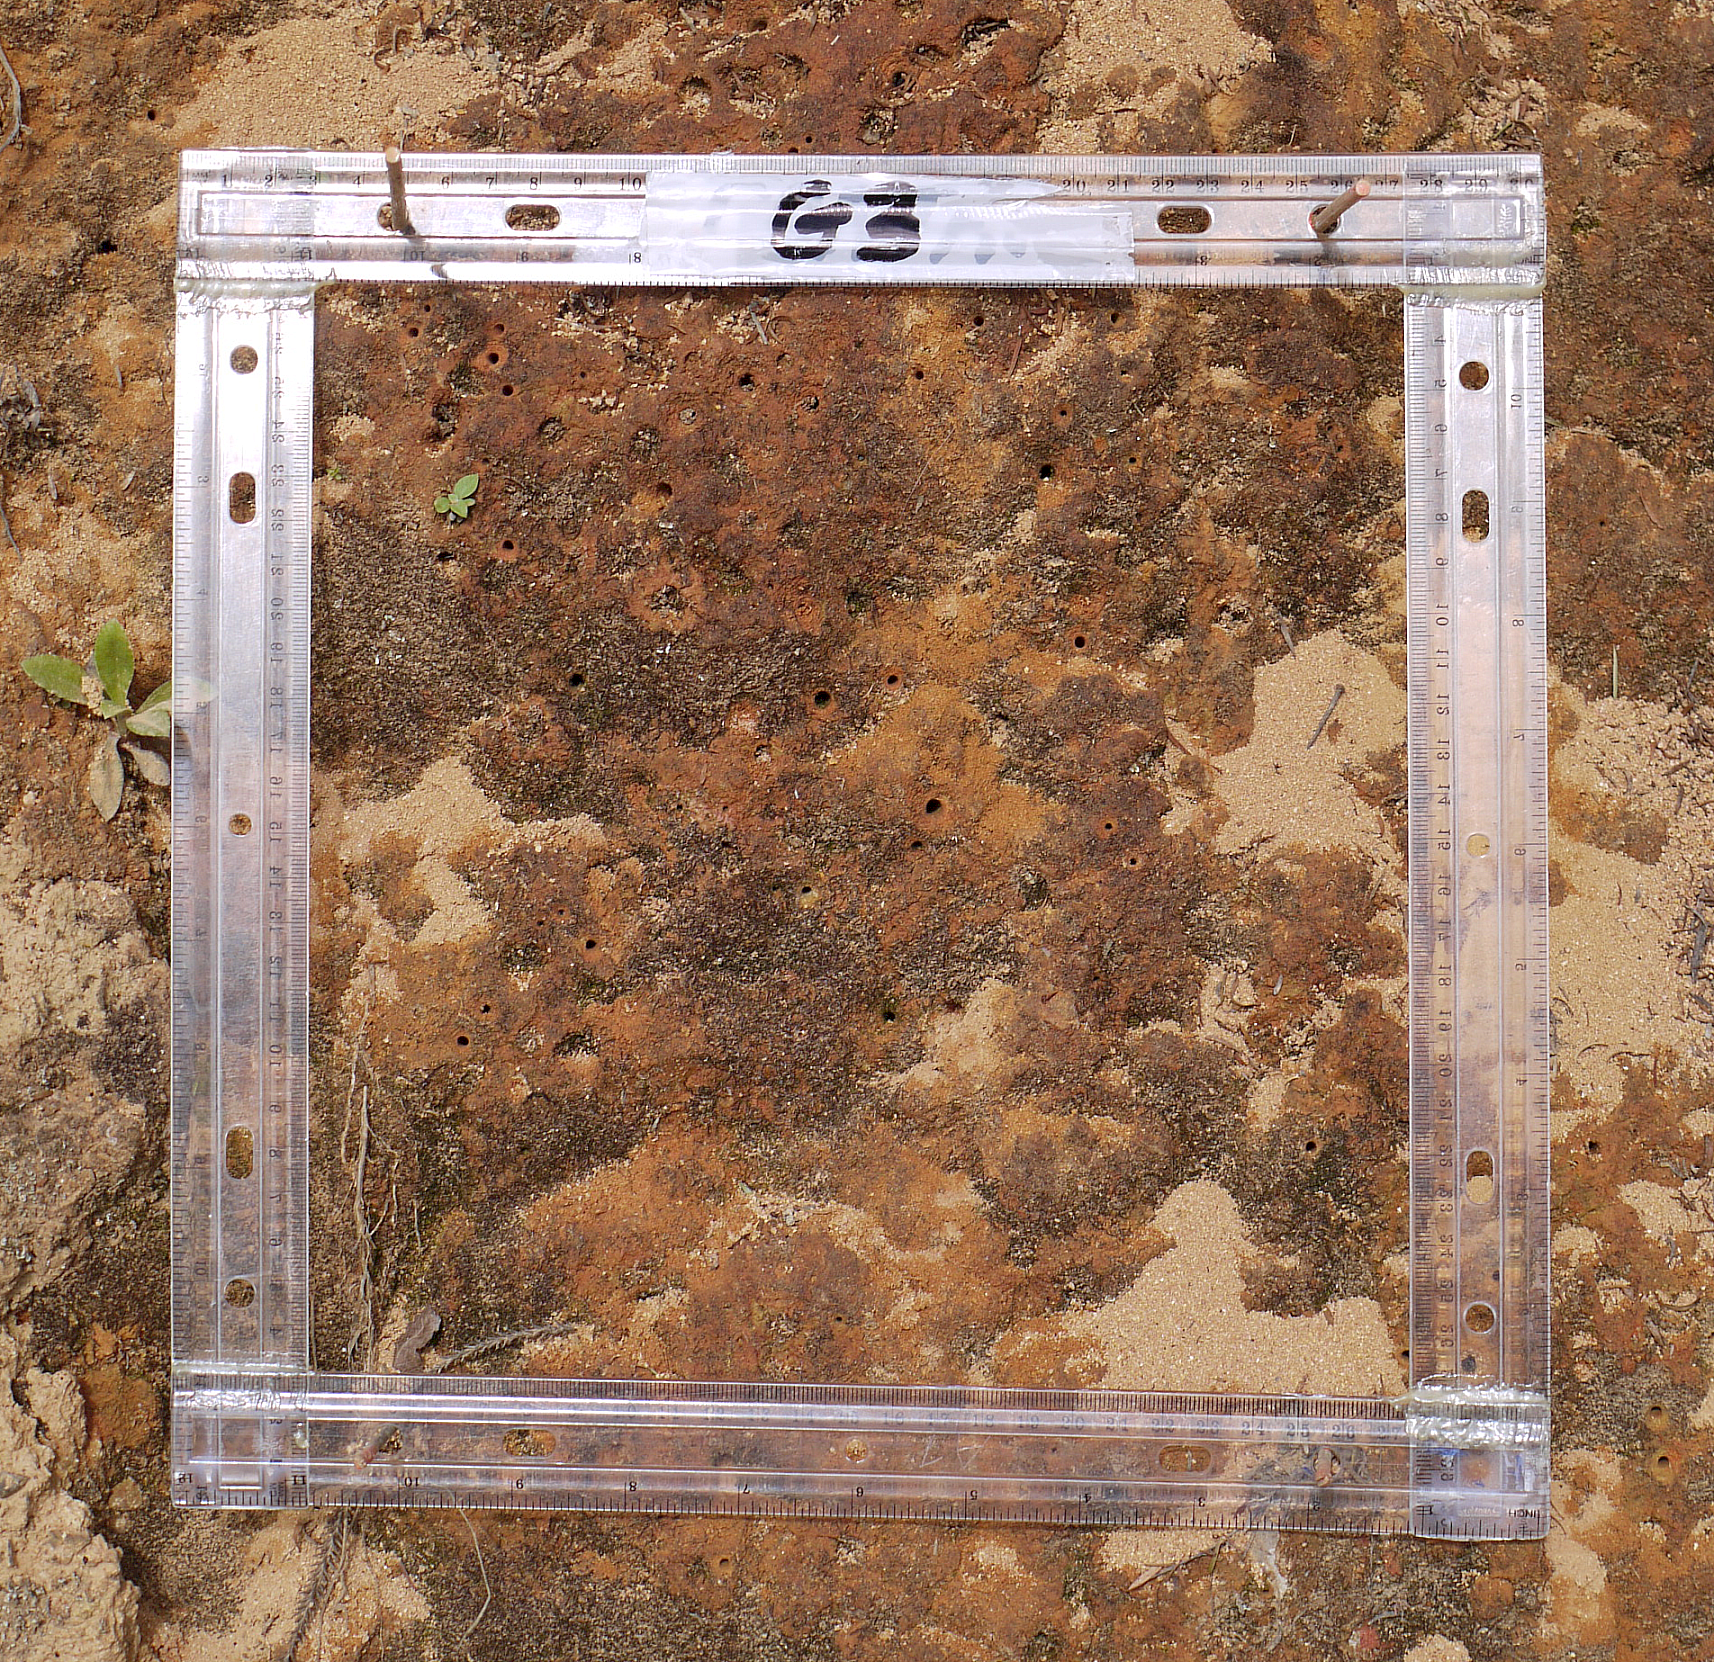
\includegraphics[width=1\linewidth]{gfx4/s1g3close}} \\
\subfloat[Wide-views of Mt. Tiger: A) grids 1-2 and B) grids 3-4. The white grids were used to collect video data.]{\includegraphics[width=1\linewidth]{gfx4/s1g1234wide}} \\
\caption[Close-up and wide views of nest sites.]{Mt. Tiger monitoring images showing (a) the set-up for grid 3 (b) the overall structure of the road-side bank .}\label{fig:wideclose-image}
\end{figure}


\begin{figure}[!htbp]\myfloatalign
\subfloat[Road-side along Memorial Drive.]{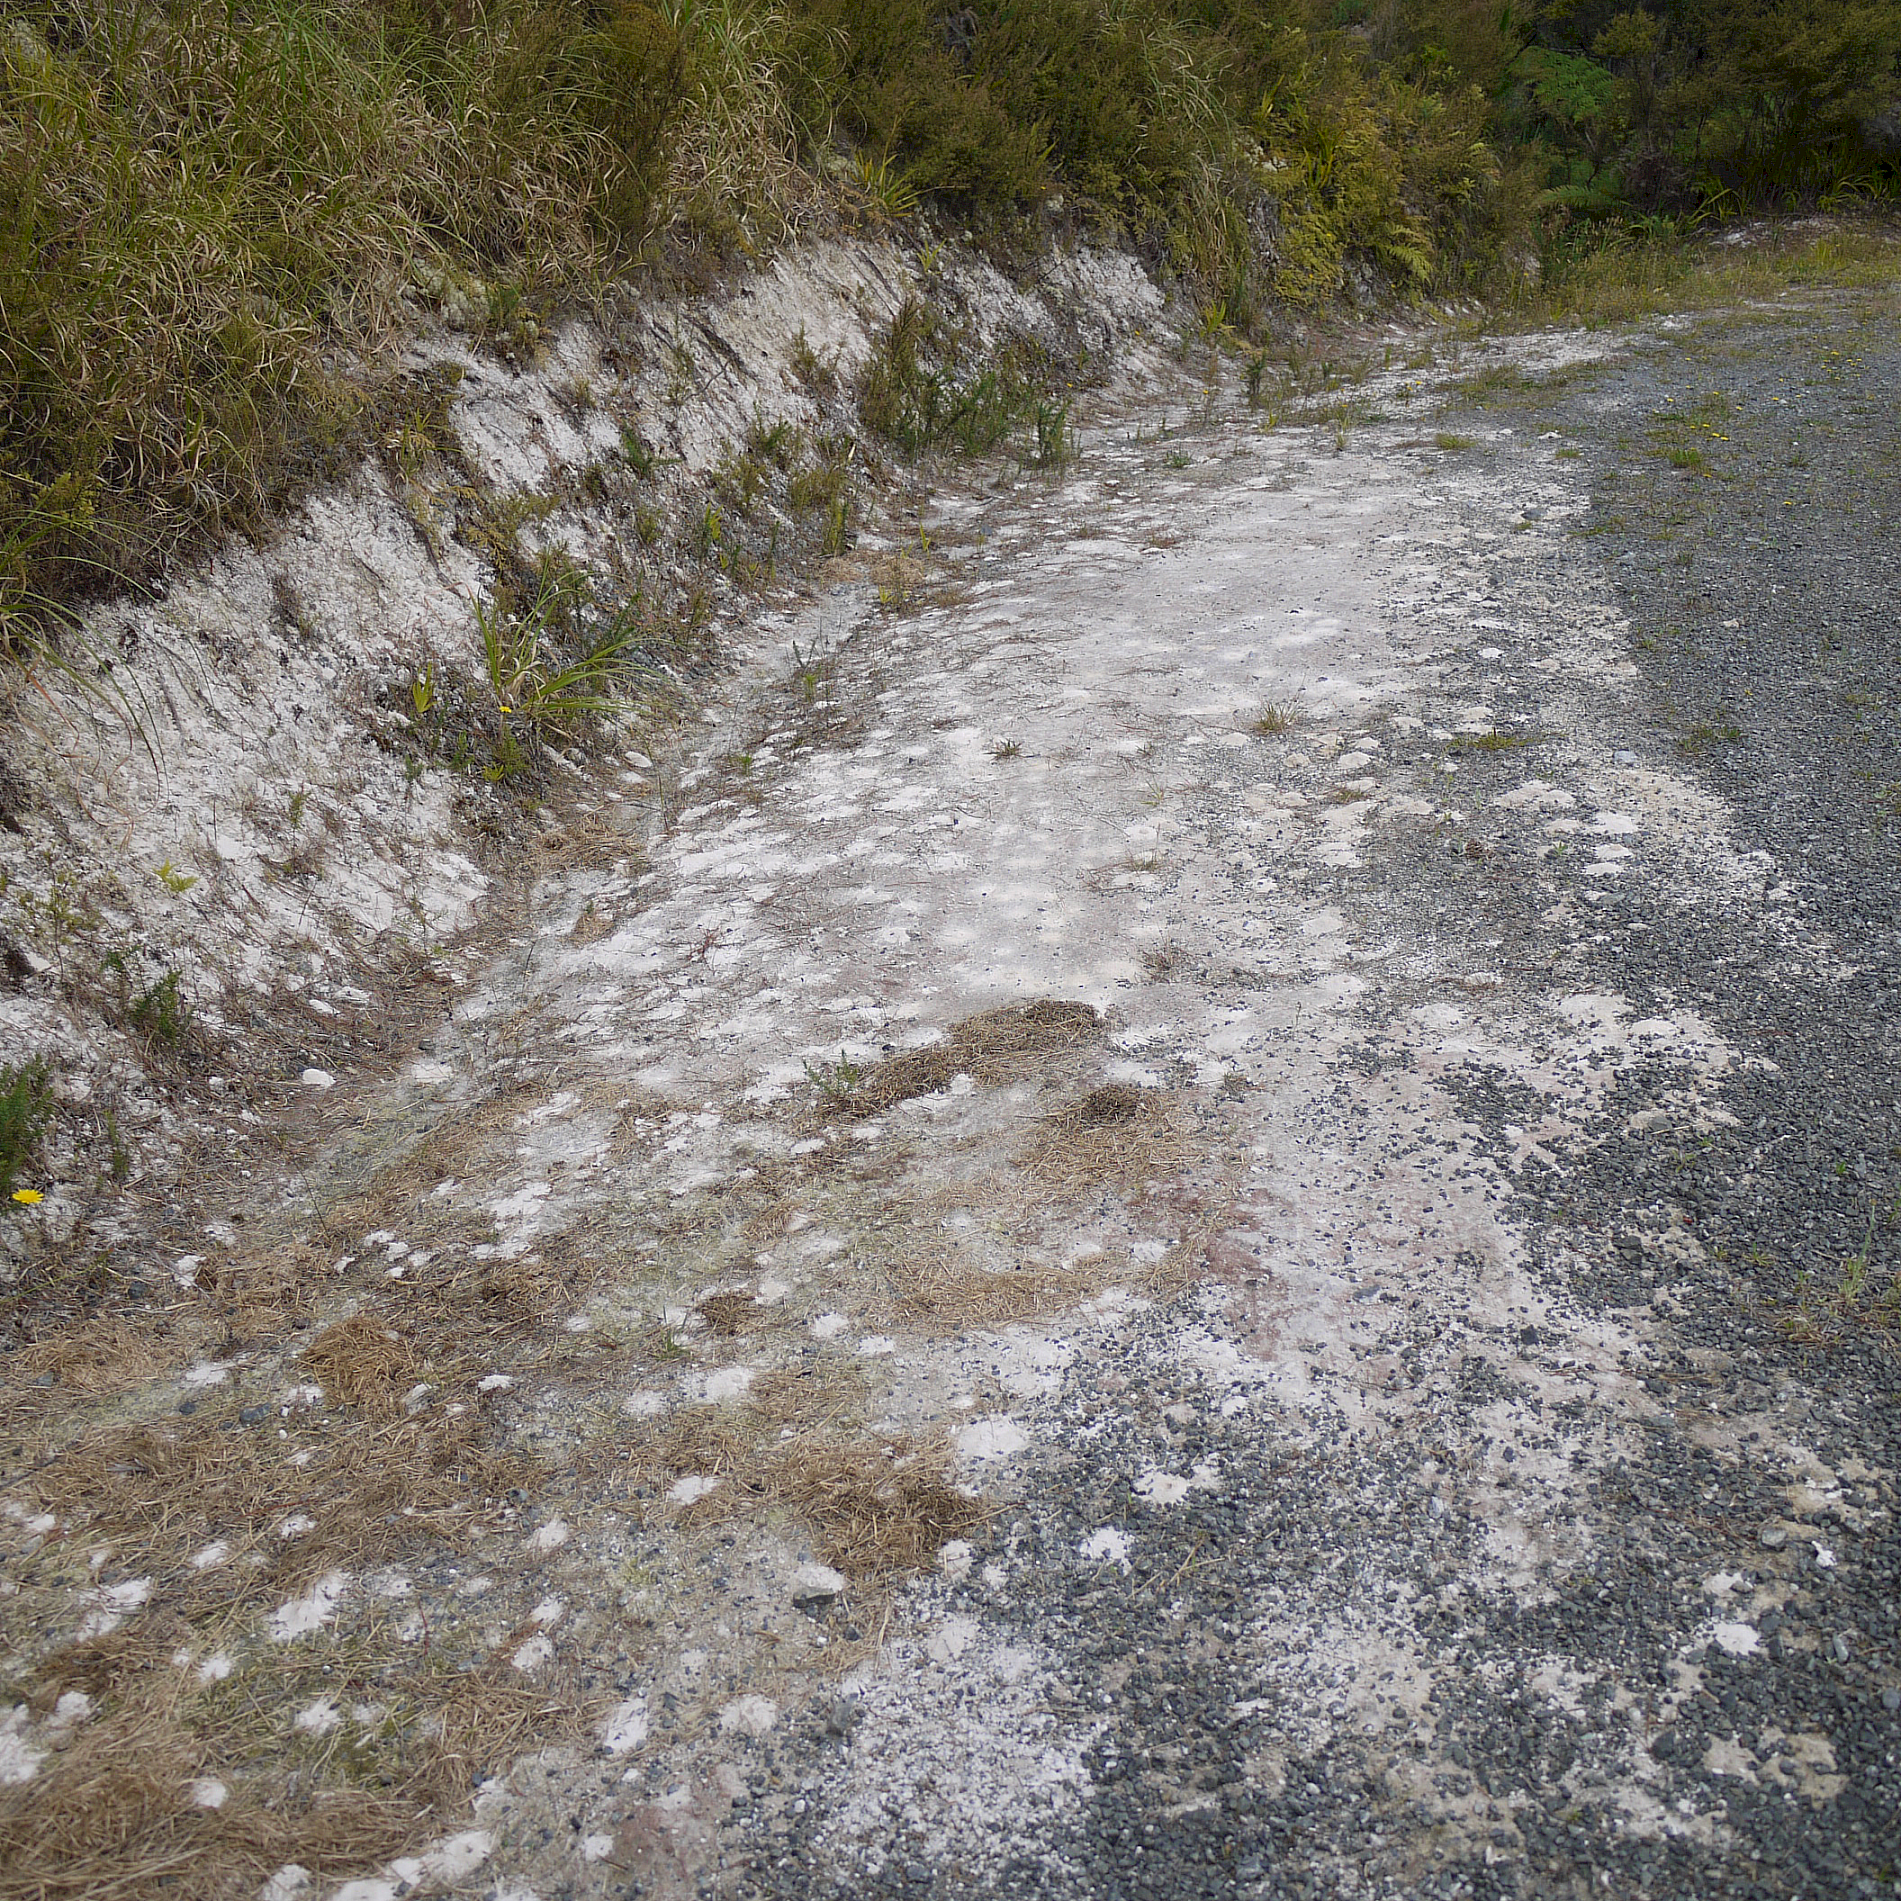
\includegraphics[width=0.47\linewidth]{gfx4/signs-memdrive}} \ \
\subfloat [Site 2: Mt. Parihaka gated area.]{\includegraphics[width=0.47\linewidth]{gfx4/signs-s2ground}} \\
\subfloat[Site 1: Tumulii in the road-side drains along Mt. Tiger ]{\includegraphics[width=0.98\linewidth]{gfx4/signs-s1roadsidedrain}} \ \
\caption[Signs marking the beginning of the active season.]{Signs marking the beginning of the active season. Mounds of white clay soil started to accumulate around horizontal ground nest entrances. This could be viably seen from a moving car, especially along (a) Memorial Drive and (b) Mt. Parihaka. The excess reddish clay soils from nest constructions could also bee seen accumulating in the roadside drains along (c) the Mt. Tiger site. }\label{fig:signs-image}
\end{figure}

\section{Summary of field methods}\label{sec:summary-of-field-methods}
Surveys were conducted over six years and monitoring data was collected across five years (2010-2014). Monitoring data were collected on each fine day, each year until there was a clear indication that bees were no longer active. The active flight season was regarded as complete when bees were no longer actively constructing nests, were not observed foraging, or were not seen in flight around their nests.

The monitoring equipment was readily acquired, low budget, off-the-shelf or easily constructed. The monitoring method was designed so the images of active nests could be collected at approximately the same time, at each location, every monitoring day. The method was consistently used each season. The image capture area was broadly estimated by using a square grid standard of measure (245 x 245 mm). Images of an artificially constructed nest and of inactive nests were acquired so they could be processed with monitoring images to help determine the accuracy of automated nest counts.

Manual counting methods have been detailed; only the entrance holes which showed signs of activity could be reliably confirmed as active. As each season progressed, the active nest entrances were increasingly more difficult to identify. Consequently the number of active nests measured on the first few monitoring days were the most important and the most reliable.

